\documentclass[10pt,letterpaper,singlecolumn]{article}
\usepackage{setspace}
\doublespacing
\usepackage{latex8}
\usepackage{times}
\usepackage{cite}
\usepackage{subfigure}
\usepackage{psfig}
\usepackage[pdftex]{graphicx}
\usepackage{epsfig}
\usepackage{pstricks}
\usepackage{fullpage}
\usepackage{amsthm}
\usepackage{graphics}
\usepackage{comment}
\usepackage[small,compact]{titlesec}
\usepackage[small,it]{caption}
\usepackage{wrapfig}

\begin{document}

\title{CSE530 Project Final Report\\
Bandwidth-Aware Memory Hierarchy Design with Hybrid Memory Technologies}

\author{Cong Xu and Jishen Zhao\\
\{czx102, juz138\}@psu.edu\vspace{-10pt}
}
\maketitle

\begin{large}

\begin{abstract}
\boldmath


\end{abstract}

% ------------------------------------------------------------------------------

\section{Introduction}

Many of modern chip-multiprocessors are designed to perform well on various
applications to achieve high performance by exploiting their inherent
parallelism. Such systems support large number of threads and single instruction
multiple data~(SIMD) execution, which puts a lot of pressure on the memory
system. Memory latency is typically not a bottleneck, since the latency can be
hidden via multi-threading or hardware prefetching. To this end, bandwidth becomes a
potential bottleneck. A high rate of computing often brings in a high rate of
data transitions. In some cases, the working set of an application fits in the
on-die caches, which can typically provide sufficient bandwidth to keep up with
the processing cores. However, if the working set does not fit in the on-die
caches, the main memory needs to provide much of the data. Since the bandwidth
of off-chip main memory is quite limited, applications with such working sets
are potentially bandwidth-bound. Therefore, it is crucial to design the memory
hierarchy to overcome the bandwidth limitation.

It is known that performance improvement of a computing system can be achieved
via multiple memory levels. Adding an extra level of memory, however, can also
help alleviate the bandwidth bottleneck of off-chip memory. Specifically, we
would like to examine (1) the number of levels in the optimal memory hierarchy,
(2) the appropriate memory technology of each level, and (3) the capacity and
bandwidth of each level. We will also explore the energy-efficiency of the
memory hierarchy design constrain, and the memory hierarchy design within a
fixed power budge.\vspace{0.15in}

% -----------------------------------------------------------------------------
\section{Motivation}

Throughput computing involves performing a huge number of calculations with a large amount of parallelism. Throughput computing applications span many domains and are already critical on a variety of platforms from high-performance computing (HPC) machines to commercial servers to client machines.

Systems designed to perform well on throughput computing applications achieve high performance by exploiting their inherent parallelism. These systems support large numbers of threads and/or use wide SIMD execution. This puts a lot of pressure on the memory system. Fortunately, memory latency is typically not a bottleneck since the latency can be hidden via multithreading or hardware prefetching, since the data access patterns are relatively simple. On the other hand, bandwidth is a potential bottleneck.

Many throughput computing applications have inherently large working sets (i.e., tens to hundreds of MB). These are unlikely to fit in conventional on-die SRAM caches for the foreseeable future. Further, unlike more traditional workloads (e.g., those similar to SPEC or TPC benchmarks), many throughput computing applications see a sharp drop in performance once caches are too small to hold their working sets. Thus, these applications are likely to be bandwidth-bound at main memory unless some significant changes are made to the memory hierarchy.

Unfortunately, there are few simple techniques to improve bandwidth efficiency of a system. While there is some work in this area~\cite{BW-Wall}, this is insufficient for the large bandwidth requirements of some throughput computing applications. So today��s systems that tout good performance for throughput computing applications (e.g., nVidia��s Tesla) do so by providing large main memory bandwidths via the use of GDDR rather than improving bandwidth efficiency. However, GDDR has fairly strict capacity limits and is much more power hungry than conventional DRAM modules. This reduces its desirability for throughput computing, and makes it a bad choice for general purpose systems trying to improve their throughput computing performance.

Emerging memory technologies such as Magnetoresistive Random Access Memory~(MRAM), Phase-Change Memory~(PCM), Resistive Random Access Memory~(RRAM),
embedded DRAM, have shown potential to to be used as on-chip caches and the main memory~\cite{Sun:2009:MRAM-L2-CMP}. Therefore, we explore how to enhance the memory hierarchy from the bandwidth point of view.


% -----------------------------------------------------------------------------

\section{Emerging Memory Technologies}

We first review the technology background three types of non-volatile memories, which are STT-RAM, PCRAM, and RRAM.

\subsection{STT-RAM}
STT-RAM uses the magnetic property of the material and uses Magnetic Tunnel Junction (MTJ) as its binary storage.  As shown in Fig.~\ref{fig:mram_cell}, MTJ contains two ferromagnetic layers and one tunnel barrier layer. The direction of one ferromagnetic layer is fixed, which is called the reference layer, while the direction of the other one can be changed by passing a driving current, which is called the free layer. The relative magnetization direction of two ferromagnetic layers determines the resistance of MTJ.  If two ferromagnetic layers have the same directions, the resistance of MTJ is low, indicating a ``0" state; if two layers have different directions, the resistance of MTJ is high, indicating a ``1" state.

\begin{figure*}[htbp]
% The "!" means to maintain the aspect ratio.
\centering
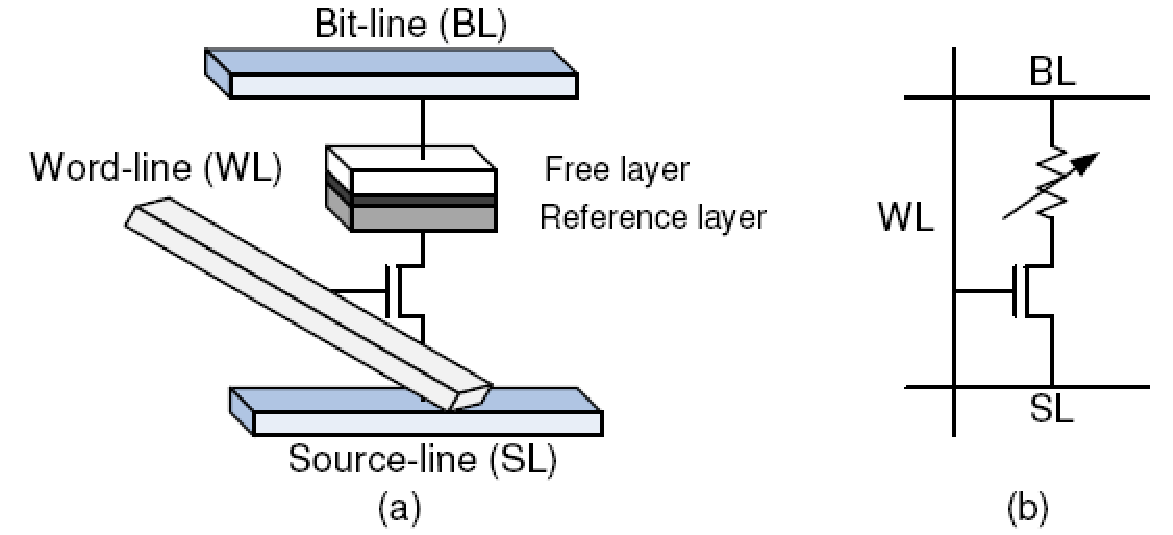
\includegraphics[width=3in]{figures/mram_cell}
\caption{Demonstration of a MRAM cell. (a) Structural view. (b) Schematic view.}
\label{fig:mram_cell}
\end{figure*}

\subsection{PCRAM}

PCRAM uses chalcogenide-based material to storage informations.  The chalcogenide-based materials in recent PCRAM research are usually alloys of germanium, antimony, and tellurium (GeSbTe, or GST), which can be switched between a crystalline phase (SET or ``1" state) and an amorphous phase (RESET or ``0" state) with the application of heat. The crystalline phase shows high optical reflectivity and low electrical resistivity, while the amorphous phase is characterized by low reflectivity and high resistivity.

\begin{figure*}[htbp]
% The "!" means to maintain the aspect ratio.
\centering
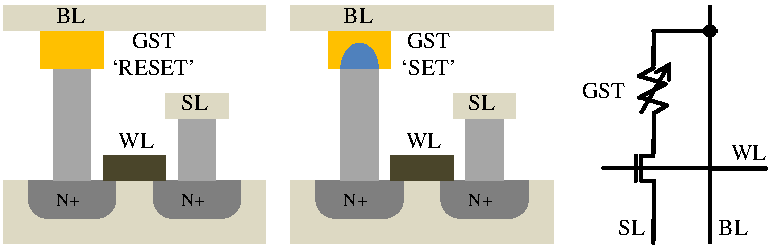
\includegraphics[width=3in]{figures/GST}
\caption{The schematic view of a PCRAM cell with MOSFET selector transistor (BL=Bitline, WL=Wordline, SL=Sourceline}
\label{fig:GST}
\end{figure*}

\subsection{RRAM}

\begin{figure*}[htbp]
% The "!" means to maintain the aspect ratio.
\centering
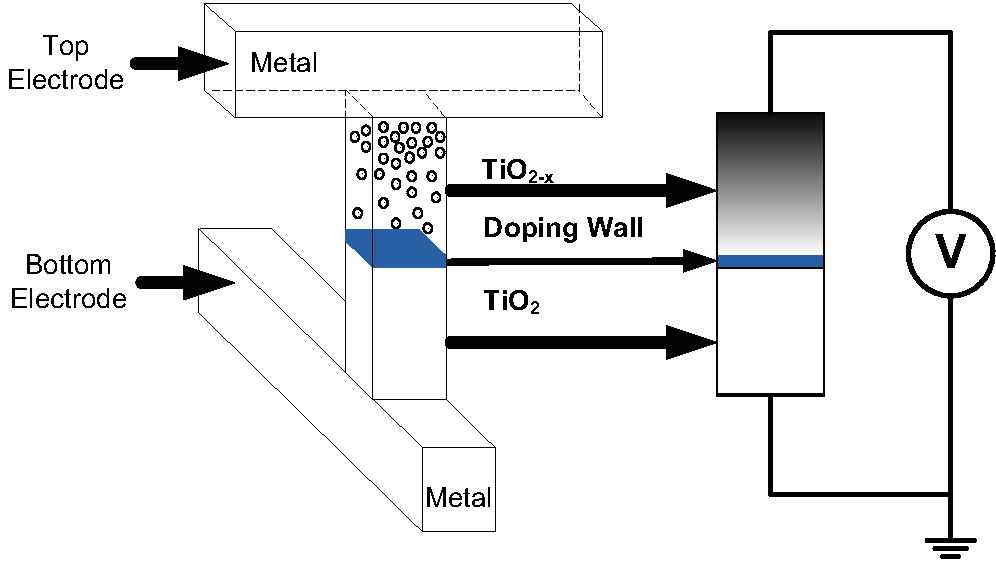
\includegraphics[width=3in]{figures/memristor}
\caption{The conceptual view of the structure of memristor cells.}
\label{fig:memristor}
\end{figure*}

Memristor, a portmanteau of ``memory resistor'', is a generalized resistance that maintains a functional relationship between the time integrals of current and voltage.  Memristor was first theoretically predicted by Chua in 1971~\cite{memristor:chua} as the fourth fundamental circuit element from the completeness of relations between the four basic circuit variables, namely, current, voltage, charge, and flux-linkage.  The first memristor practical demonstration was presented by Williams \emph{et al.} in 2008~\cite{memristor:missing}.  Fig.~\ref{fig:memristor} shows a conceptual view of the memristor structure~\cite{memristor:missing}. The top electrode and bottom electrode are two metal nanowires on platinum, and the thin titanium dioxide film is sandwiched by the electrodes.



% -----------------------------------------------------------------------------
\section{Memory Technology Pre-Exploration}
Many modeling tools have been developed during the last decade to enable system-level design exploration for SRAM- or DRAM-based cache and memory design.  For example, CACTI~\cite{CACTI} is a tool that has been widely used in the computer architecture community to estimate the speed, power, and area of SRAM and DRAM caches. In addition, CACTI has also been extended to evaluate the performance, power, and area for STT-RAM~\cite{CACTI:DAC08:Dong}, PCRAM~\cite{CACTI:GLSVLSI08:Mangalagiri,CACTI:PCRAMsim}, and NAND flash~\cite{CACTI:DATE10:Mohan}. However, as CACTI is originally designed to model SRAM-based cache, some of its fundamental assumptions do not match the actual NVM circuit implementation, and thereby these CACTI-like estimation tools do not model the NVM array organization in the exact way that the chip is fabricated. In this section, we use \emph{NVSim}, a circuit-level model for NVM performance, energy, and area estimation, which supports various NVM technologies including STT-RAM, PCRAM, RRAM, and conventional NAND flash.

\begin{figure*}[htbp]
% The "!" means to maintain the aspect ratio.
\centering
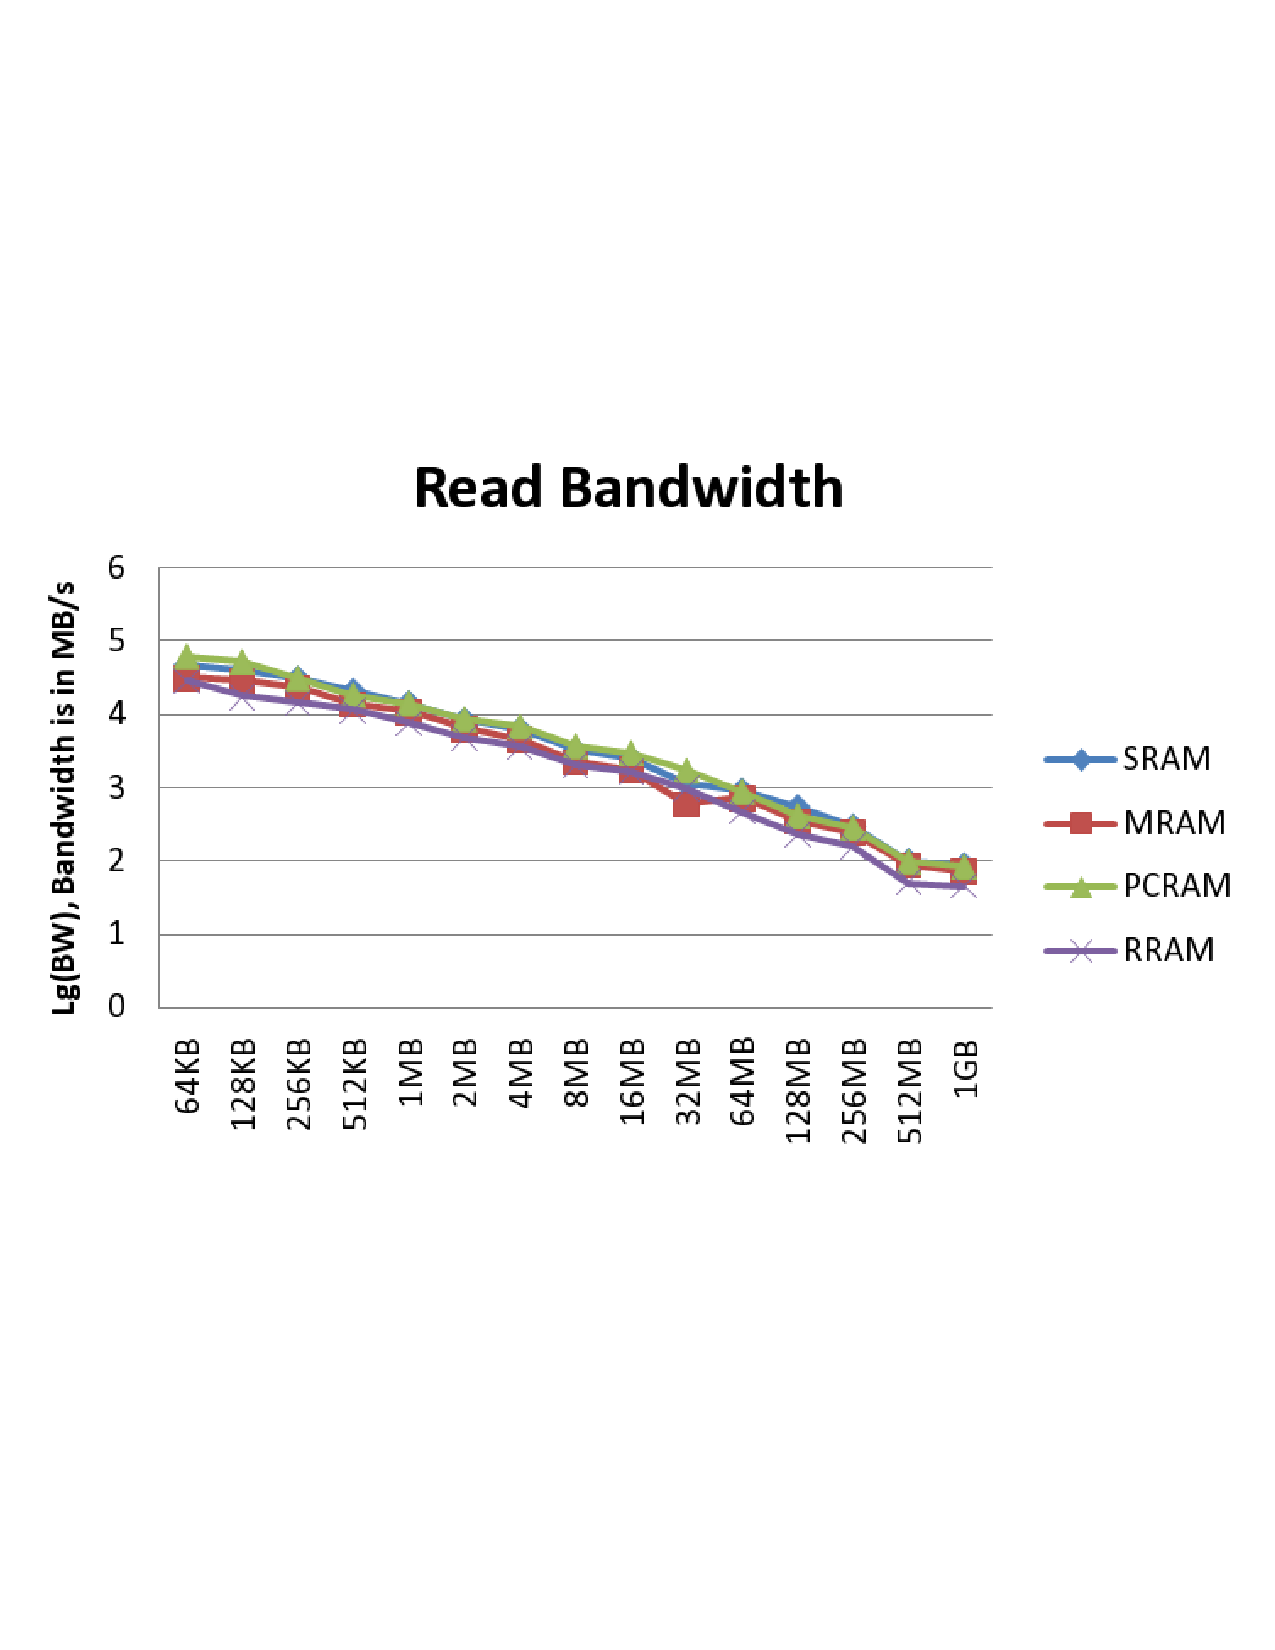
\includegraphics[width=3in]{figures/read-bw}
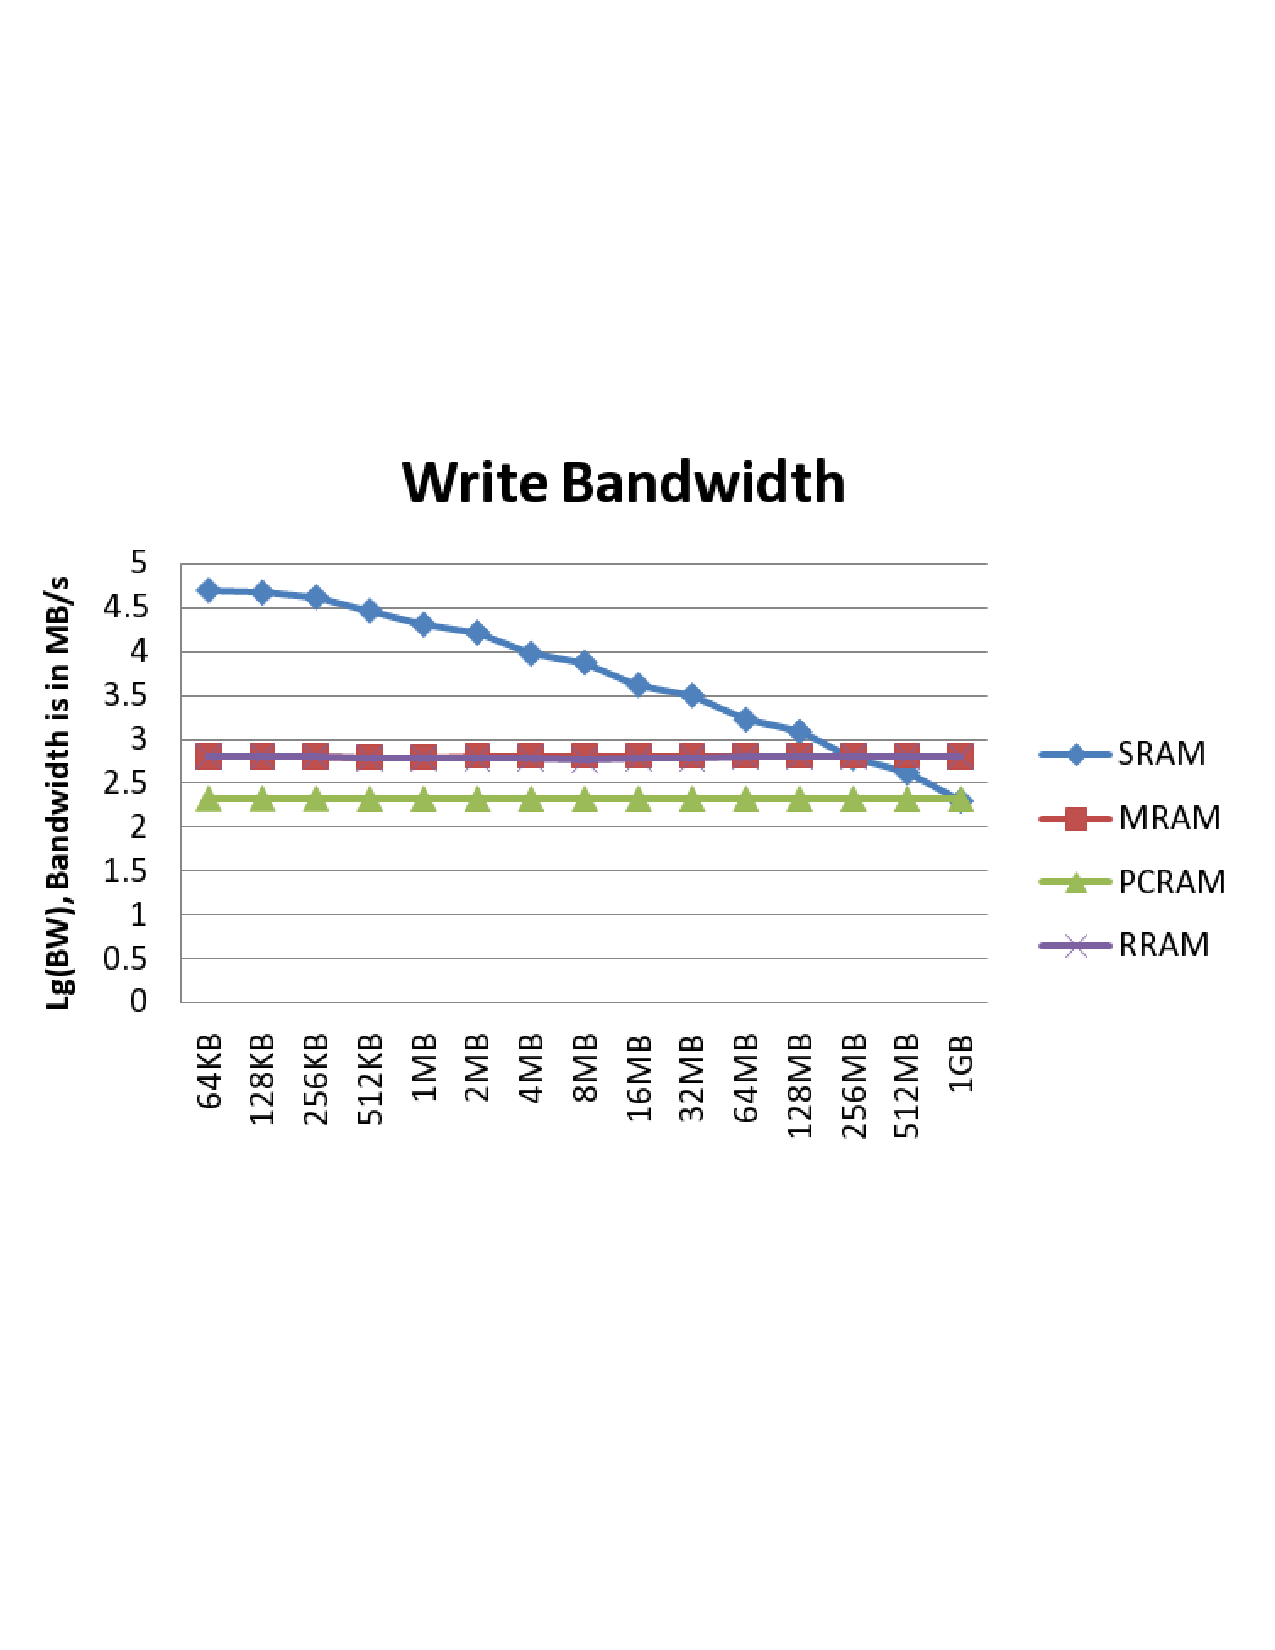
\includegraphics[width=3in]{figures/write-bw}\\

\vspace*{-1in}
\hspace{0.02in}
\makebox[3in][l]{\textcolor [rgb]{0,0,0} {\bf (a)}}
\makebox[3in][l]{\textcolor [rgb]{0,0,0} {\bf (b)}}

\caption{Read and write bandwidths provided by different memory technologies.
(a) Read bandwidth provided by different memory technologes. (b) Write bandwidth
provided by different memory technologies.}
\label{fig:memory-bw}
\end{figure*}

\begin{figure*}[htbp]
% The "!" means to maintain the aspect ratio.
\centering
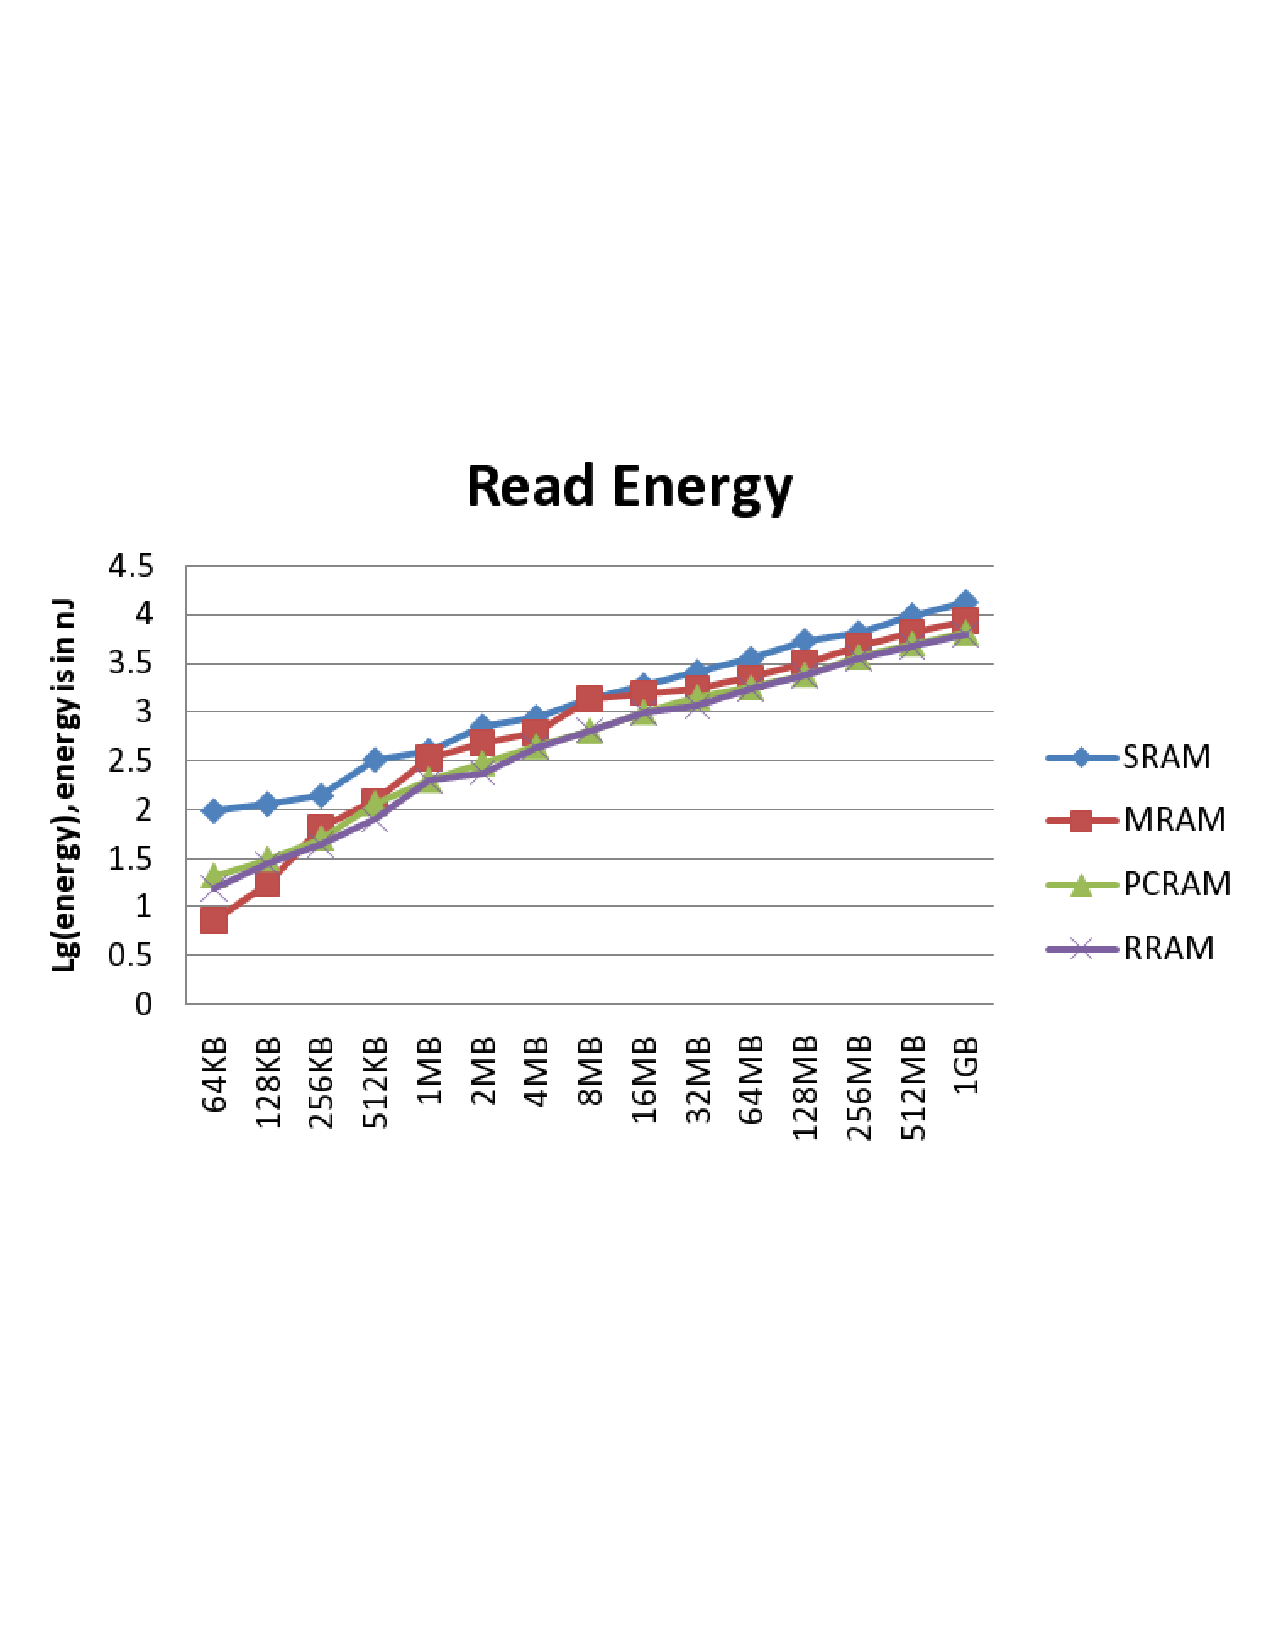
\includegraphics[width=2in]{figures/read-energy}
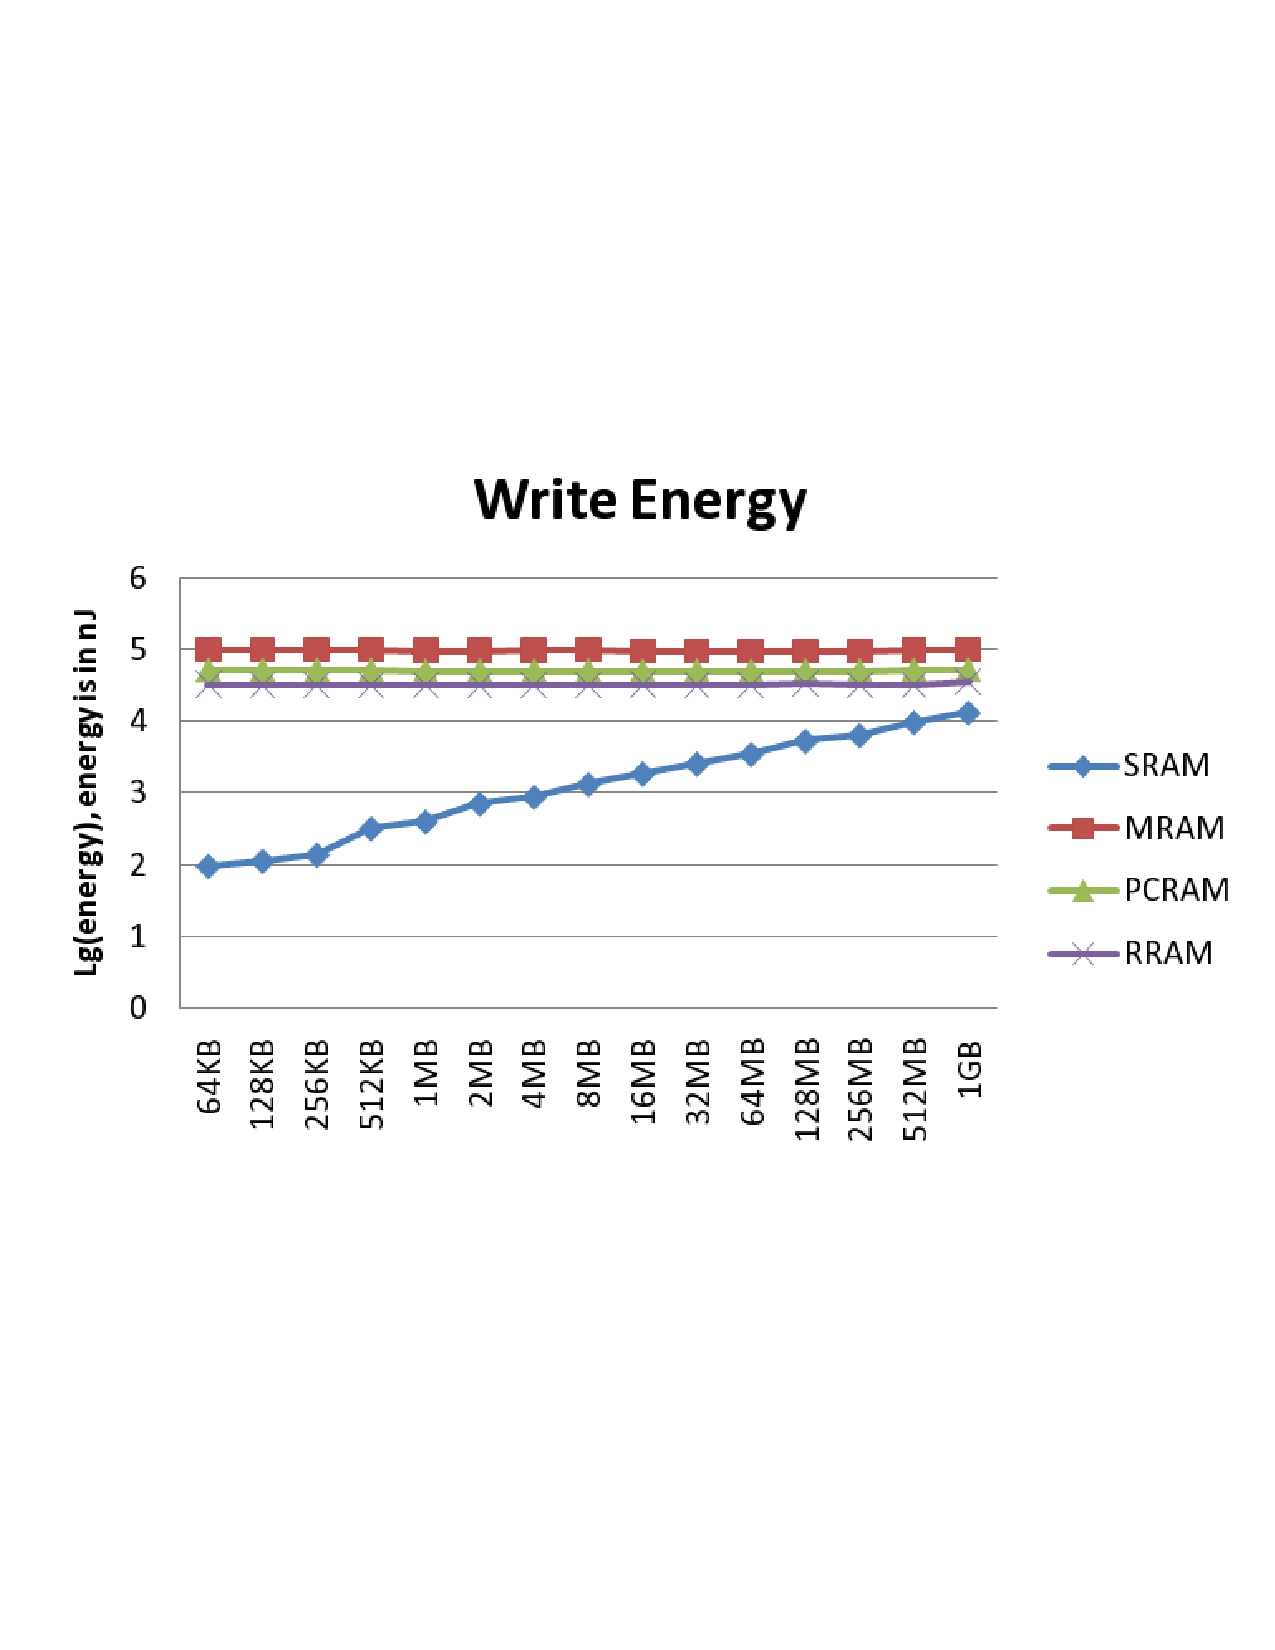
\includegraphics[width=2in]{figures/write-energy}
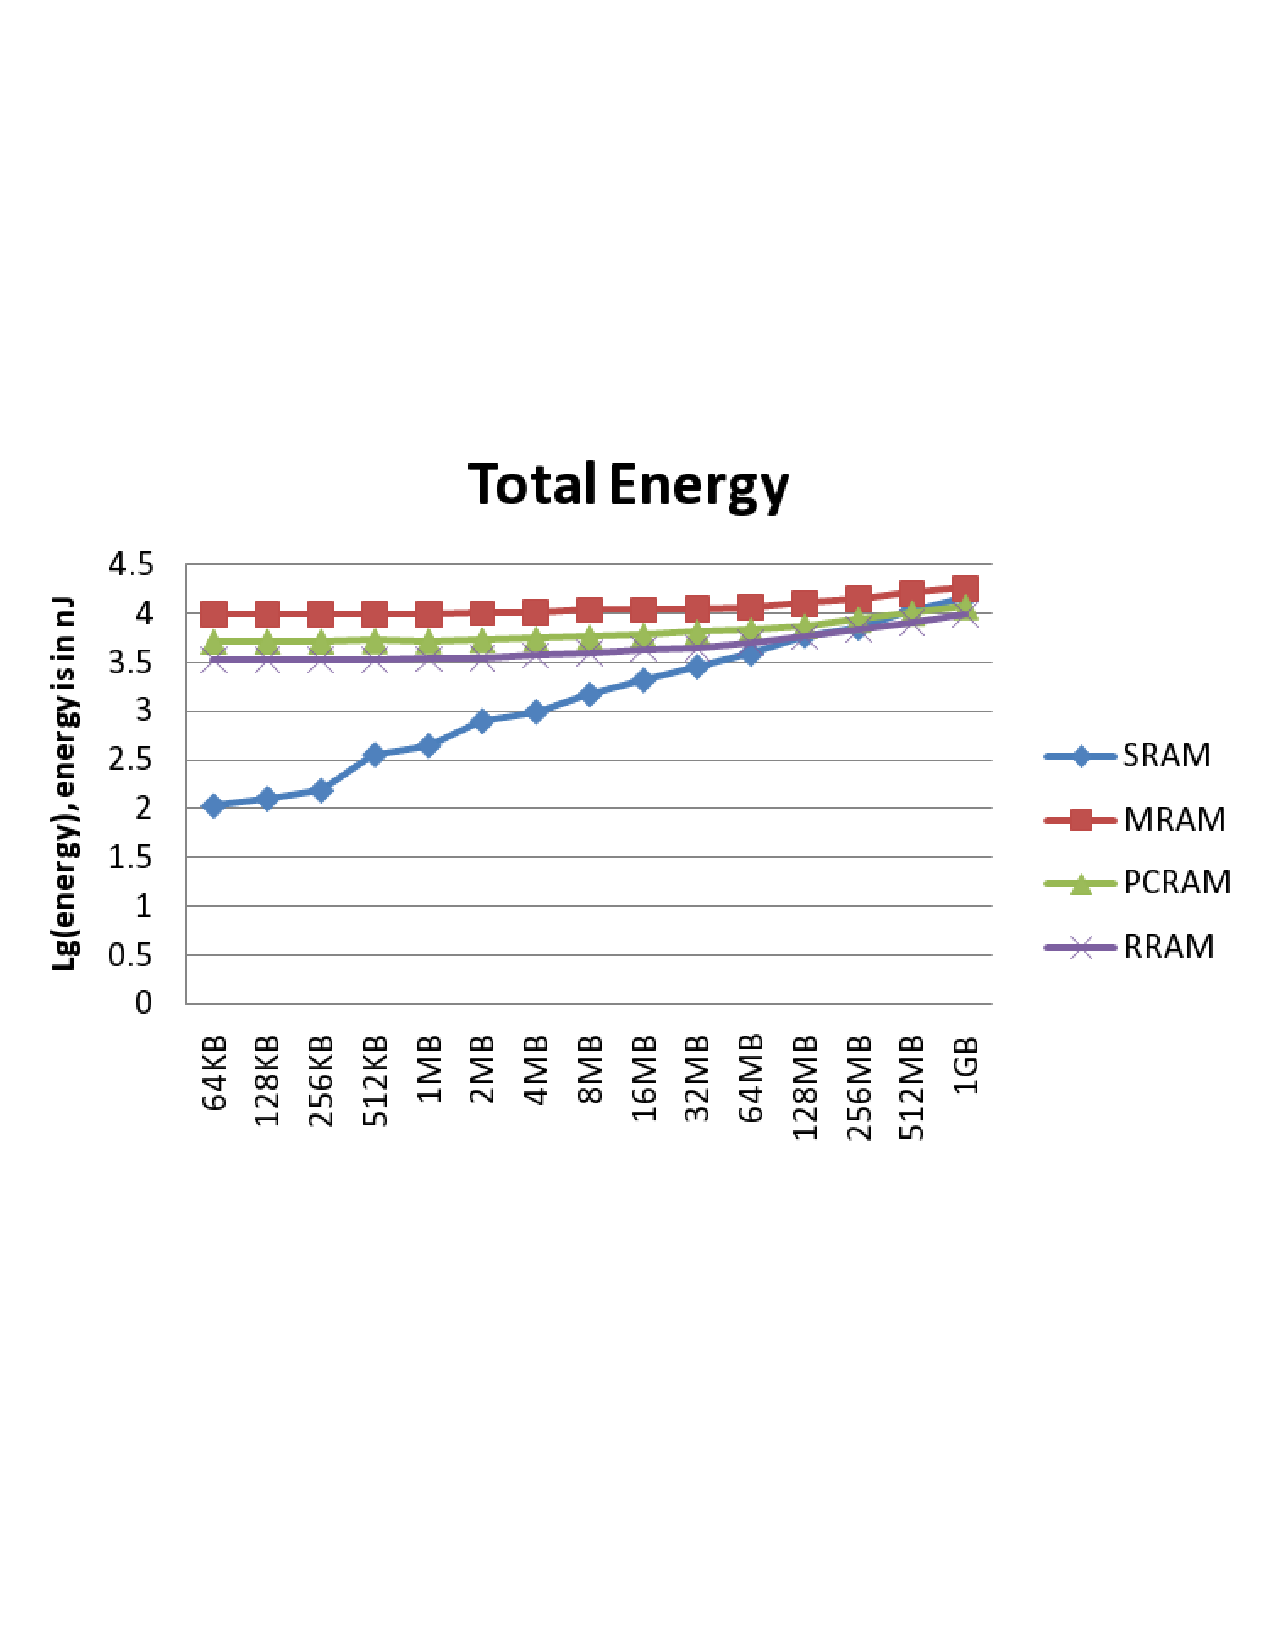
\includegraphics[width=2in]{figures/total-energy}\\

\vspace*{-0.5in}
\hspace{0.02in}
\makebox[2in][l]{\textcolor [rgb]{0,0,0} {\bf (a)}}
\makebox[2in][l]{\textcolor [rgb]{0,0,0} {\bf (b)}}
\makebox[2in][l]{\textcolor [rgb]{0,0,0} {\bf (c)}}

\caption{Dynamic energy consumption with the provided bandwidths of different
  memory technologies. (a) Read energy of different memory technologes. (b)
  Write energy of different memory technologies. (c) Total energy consumption
  (with 10\% write) of different memory technologies.}
\label{fig:memory-energy}
\end{figure*}

First of all, we estimate the read and write bandwidths that can be provided by
different memory technologies. Figure~\ref{fig:memory-bw} shows the results,
with both x- and y-values in \emph{log} scale. The figure illustrates both the
provided read and write bandwidth as a function of memory capacity. Each of the
memory technologies actually provide nearly the same read bandwidths, as is
shown in figure~\ref{fig:memory-bw}(a). On the other hand, a straight forward
observation from figure~\ref{fig:memory-bw}(b) is that the write bandwidth
varies among different memory technologies. The shape of the SRAM write
bandwidth curve is very similar to the read bandwidth curve. The write bandwidth
curves of the other three memory technologies appear to be very different. The
reason is that write latencies of the three non-volatile memories are much
higher than read latencies. Another observation from
figure~\ref{fig:memory-bw}(b) is that the curves cross to each other at
different locations. Based on these two observations, we would like to design a
bandwidth-aware hybrid memory hierarchy, which always provides the high memory
bandwidth with the given capacity. For example, we probably would like to use
1) SRAM when the memory capacity is under 256MB, 2) MRAM or RRAM between
256MB and 1GB (if only bandwidth is considered), and 3) PCRAM when the memory
cacity is over 1GB.

\section{Experiments}

 We will also use
Simics~\cite{Magnusson:2002:simics-orig-paper} as the simulator to evaluate our
design method. The benchmarks will be selected from bandwidth-bound
applications, which possibly include benchmarks from SPEC
CPU2006~\cite{SPEC:2006} and NPB~\cite{NPB}.\vspace{0.15in}

\subsection{Experimental Setup}

\subsection{Results}

\section{Conclusion and Future Work}

In addition, we would like to put an upper bound to the total dynamic energy
consumption of the memory hierarchy. Figure~\ref{fig:memory-energy} shows the
estimation of dynamic power consumptions of different memory technologies with
the provided bandwidths. In figure~\ref{fig:memory-energy}(c), we estimate the total
dynamic energy with 10\% write activities.

% \bibliographystyle{IEEEtran}
\bibliographystyle{latex8}
\bibliography{./bib/ref,./bib/reram,./bib/cacti}

\end{large}

\end{document} 